\chapter{概率}

\begin{quote}[J. C. 麦克斯韦]
我们这个世界的真正逻辑寓于概率的计算之中。
\end{quote}

\section{机会和可能性}

“机会”是日常生活中通常使用的一个词汇。无线电在播送明天的天气预报时可能会说:“明天下雨的机会是百分之六十。”你也许会说:“我能活上一百岁的机会是不大的。”科学家也使用机会这个词。一个地震学家可能会对这样的问题感兴趣:“明年在南加利福尼亚州发生某一级地震的机会有多大?”一个物理学家也许会提出这样的问题:“在下一个十秒钟内,某一特定盖革计数器将记录到20个计数的机会是多少?”一个政治家或国务活动家可能对下列问题感兴趣:“下一个十年内发生核战争的机会是多少?”同样,你也许会对从这一章中将学到一些的机会发生兴趣。

所谓\uwave{机会}指的是某种类似于猜测的事。为什么我们要猜测呢?希望作出判断而只掌握不完全的信息或不确定的知识时,我们就要进行猜测。我们要对这是些什么东西或者可能发生什么事情进行猜测。由于必须作出决定,我们常常要进行猜测。比如说,明天我是否要带上雨衣?我应设计一座能够防御哪种程度地震的新大厦?我是否要为自己建造一个放射性微粒掩蔽所?我是否要在国际谈判中改变自己的立场?我今天是否要去上课?

有时我们所以要进行猜测,是因为我们想用自己有限的知识来对某种情况说出尽可能多的东西。\textbf{事实上,任何一个判断本质上都是一种猜测。同样,任何物理理论都是一种猜测,其中有成功的,也有失败的}\footnote{这里只是简单提一下,实际上这句话蕴含了极深极丰富的哲学思想。}。概率论就是为进行较好猜测而产生的一种理论体系。应用概率的语言能使我们定量地谈论某些情况,而这些情况的变化可能很大,但确有某种一贯的平均行为。

让我们来研究向上抛掷硬币这件事。如果抛掷——以及硬币本身——都是“可靠”的,那么对任何一次特定的抛掷,我们无法预期能得到什么样的结果。然而我们可能会感到,在大量的抛掷中应该得到数目大致相等的正面和反面。我们说:“每次抛掷以正面落地的概率是0.5。”

我们只是为了对将来要做的那些观察而谈到概率的。所谓在一次观察中将得到一个特定结果的“概率”,就是指我们在大量重复这个观察时对其中出现该特定结果的最可能分数的估计。如果我们设想重复某种观察——比如看一下刚抛掷的硬币——$N$次,并且称$N_A$为我们对这些观察中最可能出现某一指定结果$A$——比如出现“正面”的数的\uwave{估计}。那么所谓观察到$A$的概率$P(A)$就是指:
\begin{equation}
\label{Eq:I:6:1}
P(A)=\frac{N_A}{N}.
\end{equation}

对我们这个定义,需要作几点注释。首先,只有当所发生的事件是某一\uwave{可重复}的观察的可能结果时,我们才能谈到发生某件事的概率。像“那所房子里出现一个幽灵的概率是多少?”这类问题有没有任何意义是不清楚的。

你可以争辩说,没有一种情况可以\uwave{不折不扣}地重复。这是对的。每一个不同的观察至少必须在不同的时间或者不同的地点进行。我们所能说的只是,对于我们想要达到的目的来说,凡是重复进行的观察应该看来似乎都是\uwave{等价的}。至少我们应当这样假定,每一次观察都在同样准备好的情况下进行,特别是在观察开始时都要带有同等程度的无知。(玩纸牌时,如果我们偷看一下对方的牌,那么我们对自己获胜的机会的估计就显然与偷看前不同!)

我们应当强调指出,式(6.1)中的$N$和$N_A$并\uwave{不}代表实际所作观察的次数。$N_A$是我们在$N$个\uwave{想像}的观察中\uwave{可能}得出结果$A$的观察的最佳\uwave{估计}。因此,概率有赖于我们的知识以及进行估计的能力。实际上有赖于我们的常识!幸运的是,常识对于许多事物都有一致程度的共同看法,所以不同的人将会作出同样的估计。然而,概率毋需是一些“绝对”的数字。既然它们与我们对事物的无知有关,那么如果我们所掌握的知识发生变化,它们也会变得不同。

你们也许已经注意到我们的概率定义中另一个相当“主观”的方面,我们把$N_A$说成是对最可能次数的一个估计……。可是这并不意味着我们\uwave{不折不扣}地期望能观察到$N_A$,而是期望能得到一个\uwave{靠近}$N_A$的数,而且数$N_A$比其邻近任何其他的数\uwave{更为可能}。比如说,我们抛掷一个硬币$30$次,那么我们可以预料,得到正面的数字不大可能正好是15,而很可能是某一靠近15的数,如12,13,14,15,16或17。然而,如果我们\uwave{必须}对之作出决择,那么我们就会决定,15次正面要比任何其他的数\uwave{更为可取}。我们将写成:P(正面)=0.5。

为什么我们选择15为一个比任何其他数更可取的数呢?我们一定会同自己以如下方式进行过争辩:如果在$N$次抛掷中得到正面的最可能次数为$N_H$,那么得到反面的最可能次数$N_T$就等于$N-N_H$。(这里我们作了这样的假定,即每次抛掷\uwave{不是}得到正面\uwave{便是}得到反面,不会得到“其他”结果! )但如果硬币是“可靠”的,它就既不偏向正面,也不偏向反面。除非有某些理由可以认为硬币(或者抛掷)是不可靠的,我们就必须认为正面与反面具有相等的可能性。所以必须使$N_T=N_H$。这样就得到$N_T=N_H=N/2$或者$P(H)=P(T)=0.5$。

我们可以把这一论证推广到任何一种情况;在这种情况下,可以观察到$m$个不同但又“相等”(即机会均等)的可能结果。如果通过观察能得到$m$个不同结果,而且又有理由相信,其中任何一个结果与别的任何结果同样可能,那么得到某一个\uwave{特定}结果$A$的概率就等于$P(A)=1/m$。

如果在一个不透明的盒子里有7个不同颜色的小球,我们“随便”(即不朝它看时)取出一个,那么得到某一种颜色的小球的概率是$1/7$。从已洗过的52张牌中“任意”抽出一张红桃10的概率是$1/52$。掷骰子而得到两个一点的概率是$1/36$。
\begin{center}
\makebox[200pt]{\hrulefill}
\end{center}

\begin{small}
从第五章中,我们用原子核的表观面积,或者称为“截面”来描写它的大小。这样做时,实际上我们就是在谈概率。当我们向一块薄的材料发射一个高能粒子时,它有一定机会直接穿过去,也有一定机会碰撞在一个原子核上。(既然原子核如此之小,以致我们无法\uwave{看到},我们就不可能直接瞄准,而必须“盲目射击”。)设在这块薄板中有$n$个原子,而每个原子的核具有截面积$\sigma$,那么被所有这些核所“遮盖”的总面积为$n\sigma$。在随机发射的很大数目$N$中,我们预期能击中\uwave{某些}核的数目$N_C$与$N$之比,犹如被遮盖的面积与薄板的总面积之比:
\begin{equation}
\label{Eq:I:6:2}
\frac{N_C}{N}=\frac{n\sigma}{A}.
\end{equation}
因此我们可以说,任何一个入射粒子在穿过薄板时将经受一次撞击的\uwave{概率}为
\begin{equation}
\label{Eq:I:6:3}
P_C=\frac{n}{A}\,\sigma,
\end{equation}
其中$n/A$是我们这块薄板中单位面积内的原子数。
\end{small}



\section{起伏}

\begin{wrapfigure}{r}{0.45\textwidth}
    \centering
    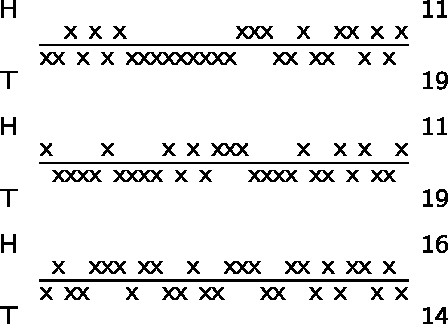
\includegraphics[width=0.35\textwidth]{Chapter6/三十次抛掷正面和反面的前后次序}
    \caption{\footnotesize 在每轮为30次抛掷的三轮游戏中所观察到的正面和反面的前后次序}
    \label{figure:三十次抛掷正面和反面的前后次序}
\end{wrapfigure}
我们现在想利用有关概率的概念来比较详细地考虑一下这样的一个问题:“如果我把一个硬币抛掷$N$次,那么预期真正会得到多少次的正面?”然而在回答这个问题之前,让我们先来看一下在这样一个“实验”中确实会发生什么情况。图6.1表示$N=30$的这样一个实验在前三"轮”中所得到的结果。

“正面”和“反面”的前后次序完全是按照它们得到时的次序排列的。第一轮得到11次正面;第二次也是11次;第三轮16次。在这三轮试验中,我们没有一回得到15次正面,是不是要对硬币发生怀疑呢?或者在这样一种游戏中,我们设想得到正面的最可能次数是15这一点错了呢?再做97轮实验,以便一共得到每回抛掷30次的实验100轮。实验的结果列在表6.1中:
\begin{table}[H]
\caption{\footnotesize 在抛掷一个硬币30次的逐轮试验中每轮所得正面的数目}
\centering
\medskip 
\begin{tabular}{p{20pt} p{20pt} p{20pt} p{20pt} p{20pt} p{20pt} p{20pt} p{20pt} p{20pt} p{20pt}}
\toprule
11 & 16 & 17 & 15 & 17 & 16 & 19 & 18 & 15 & 13     \\
11 & 17 & 17 & 12 & 20 & 23 & 11 & 16 & 17 & 14       \\
16 & 12 & 15 & 10 & 18 & 17 & 13 & 15 & 14 & 15     \\
16 & 12 & 11 & 22 & 12 & 20 & 12 & 15 & 16 & 12       \\
16 & 10 & 15 & 13 & 14 & 16 & 15 & 16 & 13 & 18       \\
14 & 14 & 13 & 16 & 15 & 19 & 21 & 14 & 12 & 15      \\
16 & 11 & 16 & 14 & 17 & 14 & 11 & 16 & 17 & 16      \\
19 & 15 & 14 & 12 & 18 & 15 & 14 & 21 & 11 & 16      \\
17 & 17 & 12 & 13 & 14 & 17 & 9  & 13 & 19 & 13    \\
14 & 12 & 15 & 17 & 14 & 10 & 17 & 17 & 12 & 11      \\    
\bottomrule        
\end{tabular}
\end{table}

\begin{wrapfigure}{r}{0.45\textwidth}
    \centering
    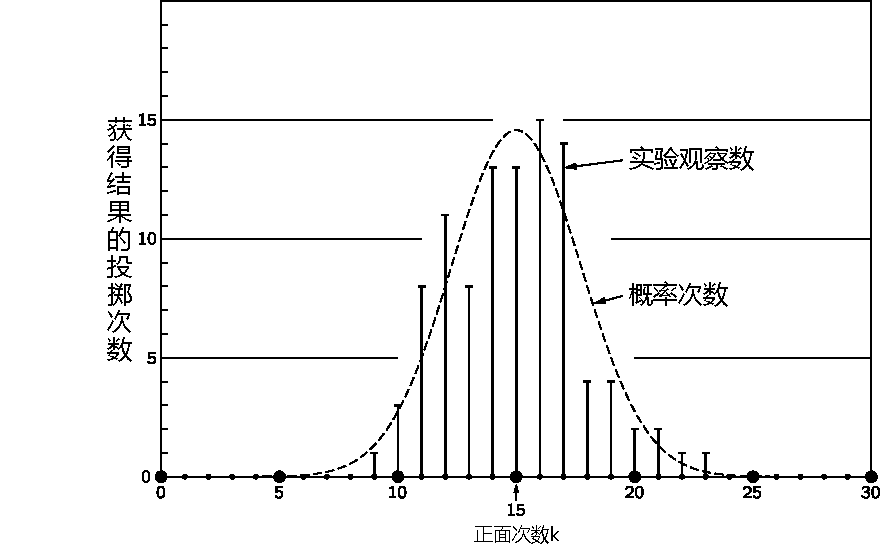
\includegraphics[width=0.43\textwidth]{Chapter6/30次抛掷的100轮游戏所得结果概况}
    \caption{\footnotesize 每轮30次抛掷的100轮游戏所得结果概况。垂直线表示记录到$k$次正面的各轮游戏的数目,虚线表示从概率计算求得的所期望记录到$k$次的游戏次数。}
    \label{figure:30次抛掷的100轮游戏所得结果概况}
\end{wrapfigure}
如果观察一下表6.1中所列出的各数,那么我们看到,大多数结果“靠近”15,而且位于12与18之间。如果我们为这些结果画一张\uwave{分布}图,那么就会对这些结果的细节有一个更好的理解。我们计算一下得到某一记录$k$的实验次数,并把这个数对每一个$k$作图,如图6.2所示,记录到15次正面的共13轮游戏,记录到14次正面的也是13轮。得到16的17次的,每一个都\uwave{大于}13轮,我们是否断定这里对正面有所偏袒?我们的" 最佳估计"2是否不够好?是不是我们现在不应该作出这个结论,即每轮30次抛掷的“最可能”记录实际上是16次正面?但是且慢!把所有各轮游戏加到一起,就总共抛掷了3000次,而获得正面的总数是1492次。可见出现正面的抛掷其比数是0.497,很接近而稍\uwave{小}于0.5。当然我们\uwave{不应}假定抛掷后得到正面的概率大于0.5!至于某\uwave{特定}的一组观察经常得到16次正面这个事实,是一种\uwave{起伏}现象,然而我们仍然预期\uwave{最可能}的正面数是15。

我们可以提出这样的一个问题:“在30次抛掷的游戏中将获得15,16,或任何其他次数正面的概率\uwave{是}多少?”我们已经说过,在抛掷一次的游戏中,得到\uwave{一次}正面的概率是0.5,得不到正面的概率也是0.5。在抛掷两次的游戏中,有\uwave{四种}可能的结果:即$HH, HT, TH, TT$。\footnote{这里H表示Head,即正面;T表示Tail,即反面。}既然这些结果中的每一个都是同样可能的,我们就推断出:(a)记录到两次正面的概率是$1/4$,(b)记录到一次正面的概率是$2/4$,(c)记录到零次的概率是$1/4$。这里有\uwave{两}种方式可以得到一次正面。但是得到两次或零次正面的方式各只有一种。

现在我们来研究抛掷3次的游戏,第三次抛掷同样可能得到一个正面或者一个反面。这里得到三次正面的方式只有一种:我们\uwave{必须}在前两次抛掷中得到两次正面,而后在最后一次中得到正面。可是这里有\uwave{三}种方式可以得到两次正面。在掷得两次正面(一种方式)后,我们可以掷出反面,或者在前两次抛掷中只掷出一次正面(两种方式)后,我们可以掷出一个正面。因此对于$3-H, 2-H, 1-H, 0-H$等记录,其同样可能的方式的数目分别为1,3,3,1。共有8种不同的可能结果。于是其概率分别为$1/8$,$3/8$,$3/8$,$1/8 $。

刚才的讨论可以用图6.3概括之。可以清楚地看到,对于更大数目的抛掷,应如何来把这个图画下去。图6.4是抛掷6次游戏的图解。

\begin{figure}[htbp]
    \centering
    \begin{minipage}[t]{0.4\textwidth}
        \centering
        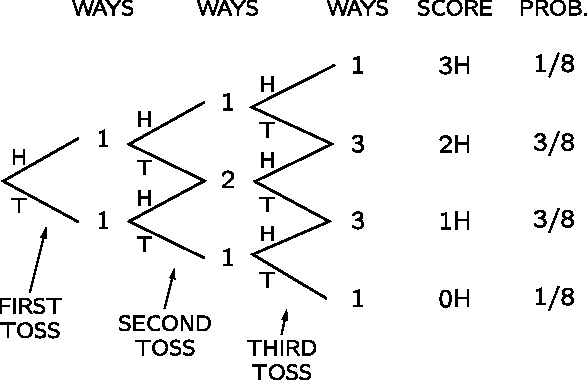
\includegraphics[width=5cm]{Chapter6/抛掷三次游戏的图解}
        \caption{\footnotesize 在抛掷三次的游戏中,能得到0,1,2,3次正面的方式数目的图解}
    \end{minipage}
    \begin{minipage}[t]{0.4\textwidth}
        \centering
        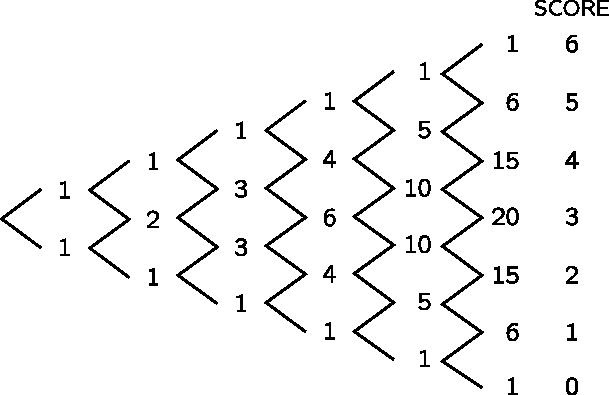
\includegraphics[width=5cm]{Chapter6/抛掷六次游戏的图解}    
        \caption{抛掷六次游戏的图解}
    \end{minipage}
\end{figure}

达到图中任何一点的所有“方式”的数目就是从起点开始到该点可以取的各种不同“途径”(即正面和反面相连的各种次序)的数目。最后一栏告诉我们掷得正面的总数。这样一种图表中出现的一组数称为\uwave{帕斯卡三角形}。这些数也称为\uwave{二项式系数},因为它们也出现在$(a+b)^n$的展开式中。如果我们称$n$为抛掷的次数,$k$为掷得正面的次数,那么图表中的数字通常用符号$\tbinom{n}{k}$来表示。顺便提一下,二项式系数也可以从式
\begin{equation}
\label{Eq:I:6:4}
\binom{n}{k}=\frac{n!}{k!(n-k)!},
\end{equation}
算出,其中$n!$称为“n阶乘”,表示连乘积$(n)(n-1)(n-2)\dotsm(3)(2)(1)$的意思。

我们现在打算根据式(6.1)来计算在$n$次抛掷中得到$k$次正面的概率$P(k,n)$。所有可能结果的总数是$2^n$(因为对每一抛掷有两个结果),得到$k$次正面的总共有$\tbinom{n}{k}$种,而每一种都是同样可能的,所以我们有
\begin{equation}
\label{Eq:I:6:5}
P(k,n)=\frac{\tbinom{n}{k}}{2^n}.
\end{equation}

既然$P(k,n)$是我们期望会得到$k$次正面的比数,那么在100轮游戏中,我们应预期共有$100\cdot P(k,n)$轮会出现$k$次正面。图6.2中虚线所经过的各点就是从$100 \cdot P(k,30)$计算出来的那些点子。我们可以看到,我们\uwave{预期}有14或15轮游戏会记录到15次正面,然而只有13轮游戏观察到这个记录,我们\uwave{预期}有13或14轮游戏会记录到16次正面,但是只有16轮游戏观察到这个记录。这样一种起伏情况实际上就是“这种游戏的组成部分”。

我们刚才用过的方法,可以应用于最一般的情况,也就是在单独一次观察中只能得出两种可能结果的情况。我们用$W$[表示“win”(赢)]和$L$[表示“lose”(输)]来表示这两种结果。在一般情况下,单独一个事件会得$W$或$L$的概率是毋需相等的。设$p$为得到结果$W$的概率,于是$q$——这个得到结果$L$的概率必然等于$(1-p)$。在一组$n$轮的试验中,得到$k$次结果为$W$的概率$P(k,n)$就等于
\begin{equation}
\label{Eq:I:6:6}
P(k,n)=\tbinom{n}{k}p^kq^{n-k}.
\end{equation}

这个概率函数称为\uwave{伯努利}或\uwave{二项式}概率。


\section{无规行走}

另一个有趣的问题也需要用到概率概念,这就是“无规行走”的问题。在最简单的形式下,我们可以想象这样一个“游戏”,其中“游戏者”从$x=0$的一点出发,要求他每“移动”一次\uwave{要末}朝前(向$+x$方向)走一步\uwave{要末}朝后(向$-x$方向)走一步。而朝前朝后必须\uwave{随机}决定,例如用抛掷硬币的方法。我们将怎样来描写这种行动的结果呢?在一般形式下,这个问题与气体中原子(或其他粒子)的运动,即布朗运动有关,也与测量中误差的组合有关。你们将会看到,无规行走问题与我们已讨论过的抛掷硬币问题密切有关。

首先,让我们看几个无规行走的例子。我们可以用行走者在$N$米中所经过的净距离$D_N$来表示他的进度。图6.5为无规行走者所走路径的三个例子。(这里我们用图6.1所示抛掷硬币所得的结果作为随机选择的移动取向。)

\begin{wrapfigure}{r}{0.45\textwidth}
    \centering
    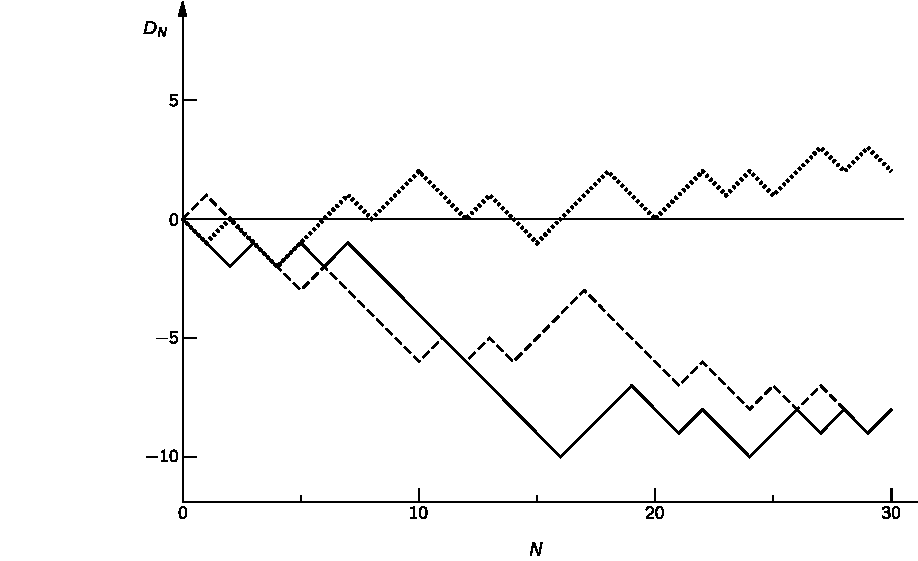
\includegraphics[width=0.35\textwidth]{Chapter6/无规行走取得的进度}
    \caption{\footnotesize 无规行走取得的进度。横座标$N$表示所走的步子总数;纵座标$D_N$表示离开起点的净距离}
    \label{figure:无规行走取得的进度}
\end{wrapfigure}

对于这样一种运动我们可以说些什么呢?首先我们也许会问:“平均而言他走了多远?”我们必定\uwave{预期}他的平均进度为零,因为他向前或向后走的可能性是均等的。然而我们似乎有这样的感觉,认为随着$N$的增加,他更可能偏离起点越来越远。因此我们也许要问,走过的用\uwave{绝对值}表示的平均距离是多少,也就是说$\abs{D}$的平均值是多少。可是在这里用另一个量度“进度”的方法更为方便,这就是用距离的平方$D^2$来表示,它无论对正的还是负的移动都为正,所以它是这种随机漫步的一个合理\uwave{量度}。

我们可以证明,$D_N^2$的预期值恰好是所走步子的数目$N$。所谓“期望值”,指的是可几值(也就是我们的最佳猜测),我们可以把它看作是对重复多次的一系列行走所\uwave{预期}的平均行为。我们用$\left <D_N^2 \right >$来表示这样一个预期值,并且也可以称它为“平均平方距离”。走一步后的$D^2$总是$+1$,所以当然$\left < D_1^2 \right >=1$。(所有的距离都将以一步为单位来量度。以后我们将不再写出距离的单位。)

当$N>1$时,预期值$D_N^2$可以从$D_{N-1}$求得。如果走了$(N-1)$步后,我们得到$D_{N-1}$,那么经过$N$步后,就有$D_N=D_{N-1}+1$\uwave{或}$D_N=D_{N-1}-1$。其平方为
\begin{equation}
\label{Eq:I:6:7}
D_N^2=
\begin{cases}
D_{N-1}^2+2D_{N-1}+1,\\[2ex]
\quad\qquad\textit{或}\\[2ex]
D_{N-1}^2-2D_{N-1}+1.
\end{cases}
\end{equation}
对于大量独立的无规行走,我们所能预期得到的,每次只有每一个数值的一半,因此我们的平均期望值恰好是这两个可能值的平均值。于是$D_N^2$的预期值就是$D_{N-1}^2+1$。\uwave{一般而言},我们对$D_N^2$所应\uwave{期望}的“期望值”就是$\left <D_{N-1}^2 \right >$(根据定义!)。所以
\begin{equation}
\label{Eq:I:6:8}
\left < D_N^2 \right >=\left < D_{N-1}^2 \right >+1.
\end{equation}

我们已经说明$\left < D_1^2 \right > = 1$;因而得到
\begin{equation}
\label{Eq:I:6:9}
\left < D_N^2 \right > =N,
\end{equation} 
这是一个多么简单的结果!

如果我们希望得到的不是距离的平方,而是像距离那样的一个数,以表示无规行走中“所作的从原点算起的进展”,那么我们可以用“方均根距离”$D_{\text{rms}}$来表示:
\begin{equation}
\label{Eq:I:6:10}
D_{\text{rms}}=\sqrt{\left < D^2 \right > }=\sqrt{N}.
\end{equation}

我们已经指出,无规行走问题在数学形式上与本章开始时讨论过的那种抛掷硬币的游戏十分相似。如果我们设想每一步的取向对应于抛掷硬币中出现的正面或反面,那么$D$正好是获得正面的次数与获得反面的次数的差值$N_H-N_T$。由于$N_H+N_T=N$是总的所走步数(或总的所抛掷次数),我们就有$D=2N_H-N$。以前我们曾为预期的分布$N$(也称为$k$)导出一个表达式,而且得到了如式(\ref{Eq:I:6:5})所示的结果。由于$N$正好是一个常数,所以我们就为$D$得到一个相应的分布。(由于超过$N/2$后出现的每次正面都会使反面受到“损失”,所以在$N_H$与$D$之间相差一个因子$2$。)图\ref{figure:30次抛掷的100轮游戏所得结果概况}表示在无规行走30步的例子中可能得到的距离分布情况。(其中$k=15$应读作$D=0$;$k=16$应读作$D=2$;等等。)

$N_H$和它的预期值$N/2$的偏差为
\begin{equation}
\label{Eq:I:6:11}
N_H-\frac{N}{2}=\frac{D}{2}.
\end{equation}

均方根(rms)偏差为
\begin{equation}
\label{Eq:I:6:12}
\biggl(N_H-\frac{N}{2}\biggr)_{\text{rms}}=\tfrac{1}{2}\sqrt{N}.
\end{equation}

根据我们对$D_{rms}$求得的结果,在走30步所预期的“典型”距离应是$D_{rms}=\sqrt{N}=\sqrt{30}=5.5$,或者典型的$k$应与$15$相差大约$5.5/2 \approx 2.8$个单位。在图\ref{figure:30次抛掷的100轮游戏所得结果概况}中,我们可以看到,从中心量起的曲线“宽度”正好大约等于3个单位,和上述结果相一致。

现在我们已有条件来考虑一直到目前为止被我们回避的一个问题。我们怎样知道一块硬币是“可靠的”或是“灌了铅的”?现在我们至少能够为之提供一部分答案。对于一块可靠的硬币,我们预期其能出现正面的次数的比值是0.5,亦即
\begin{equation}
\label{Eq:I:6:13}
\frac{\left < N_H \right > }{N}=0.5.
\end{equation}

我们\uwave{也}预期实际的$N_H$将偏离$N/2$大约有$\sqrt{N}/2$,或者说,它的\uwave{比值}与1/2的偏差为
\begin{equation*}
\frac{1}{N}\,\frac{\sqrt{N}}{2}=\frac{1}{2\sqrt{N}}.
\end{equation*}
$N$越大,所\uwave{预期}的比值$N_H/N$就越接近于二分之一。

\begin{wrapfigure}{r}{0.45\textwidth}
    \centering
    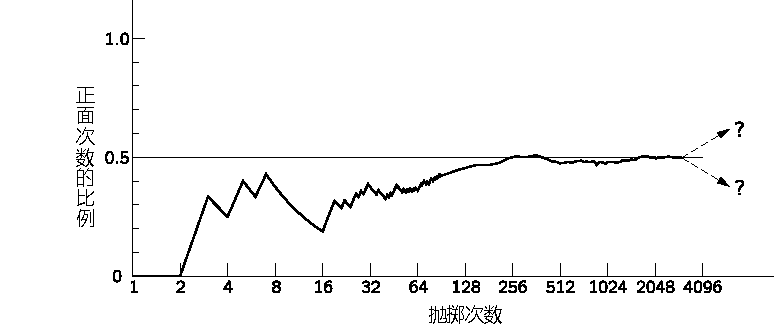
\includegraphics[width=0.35\textwidth]{Chapter6/获得正面的那些抛掷在某一特定次序中的比值}
    \caption{获得正面的那些抛掷在某一特定次序中的比值}
    \label{figure:获得正面的那些抛掷在某一特定次序中的比值}
\end{wrapfigure}
在图6.6中,我们根据本章前面提到的掷币记录画了一条表示比值$N_H/N$的曲线。从图中可以看出,对于大的$N$,得正面的比值趋向于接近0.5。遗憾的是,对任何给定的一轮或几轮,连观察到的偏差都\uwave{保证不了接近于预期}的偏差,总是有一定的机会出现大的起伏——一长串的正面或者一长串的反面——造成一个任意大的偏差。我们一切所能说的,只是\uwave{如果}偏差接近于预期的$1/2\sqrt{N}$(比如说在2或3倍之内),那么就没有理由去怀疑硬币的可靠性。如果偏差大很多,那么我们可以对硬币发生怀疑,但无法证明它是灌过铅的(或者抛掷者是非常机灵的!)。

我们也没有考虑过应该如何来处理这样一块“硬币”或某一与之相似的“不确定的”物体(比如一块始终以两种方位中无论那一种着地的石块),对于它们来说,我们很有理由认为出现正面和反面的概率应该是不同的。我们已经定义了$P(H)=\left < N_H \right >/N$。那么怎样知道$N_H$的\uwave{预期值}是多少呢?在某些情况下,我们所能做得最好的,就是去观察在大量抛掷中所得正面的数目。由于缺少任何更好的证据,我们不得不令$\left < N_H \right > = N_H\textrm{(观察值)}$。(除此之外,还能期望做什么呢?)然而必须理解到,在这样一种情况下,不同的实验或不同的观察者可能会推论出不同的概率$P(H)$。但是我们可以\uwave{预料},这些不同的答案应该在偏差$1/2\sqrt{N}$的范围内相互一致[加入$P(H)$接近于二分之一的话]。实验物理学家常常这样说:“实验确定的”概率是有“误差”的,并且把它写成
\begin{equation}
\label{Eq:I:6:14}
P(H)=\frac{N_H}{N}\pm\frac{1}{2\sqrt{N}}.
\end{equation}
在这样一个表达式中含有下列意义:\uwave{存在}着一个“真正的”或“正确的”概率,只要我们知道的东西足够多,就能把它计算出来,其次是由于有起伏,观察会发生“误差”。然而没有办法能使这种想法做到逻辑上始终如一。如果能领悟到下列几点或许要比较好一些,即概率概念在某种意义上是主观的,它总是建立在不肯定的知识上的,而且他的总量值是随着我们得到的信息越多而改变着的。


\section{概率分布}

我们现在回到无规行走的问题上来,并且考虑它的一种修正。我们设想除了每一步的方向(+或-)可以随机选择外,每一步的\uwave{长度}也能以某种无法预定的方式变化着,唯一的条件就是\uwave{平均而言}步子的长度是一个单位。这种情况更能代表像气体中一个分子的热运动那样的状况。如果我们称一步的长度为$S$,那么$S$完全可以取任何一个值,但最通常的是“接近于”1。为明确起见,我们令$\left < S^2 \right > = 1$,或者与之同等,$S_{\text{rms}}=1$。$\left < D^2 \right > $的推导将仿照以前一样,只是式(\ref{Eq:I:6:8})现在要加以改变而读作
\begin{equation}
\label{Eq:I:6:15}
\left < D_N^2 \right >=\left <D_{N-1}^2\right >+\left <S^2\right >=\left <D_{N-1}^2\right >+1.
\end{equation}

同以前一样,我们得到
\begin{equation}
\label{Eq:I:6:16}
\left <D_N^2\right > =N.
\end{equation}

现在对于距离$D$,我们会预期得到什么样的一种分布呢?比如在走了30步后,$D=0$的概率是多少?回答是$0$!$D$取\uwave{任一特定值}的概率是0。因为根本没有一种机会能使后退的(长度是变化的)步子的总和与朝前的步子的总和正好相等。我们无法画出一张像图6.2那样的图。

然而如果我们不是去问获得其值正好等于0, 1,或2的那些$D$的概率是多少,而代之以去问获得其值\uwave{靠近}0, 1,或2的那些$D$的概率有多大,那么我们就能得到与图6.2相似的曲线。我们定义$P(x,\Delta x)$为$D$位于$x$处一个间隔$\Delta x$(比如从$x$到$x+\Delta x$)内的概率。对于小的$\Delta x$,我们可以预期$D$位于这个间隔内的概率,与间隔的宽度$\Delta x$成正比。因此我们可以写成
\begin{equation}
\label{Eq:I:6:17}
P(x,\Delta x)=p(x)\,\Delta x.
\end{equation}
函数$p(x)$称为\uwave{概率密度}。

$p(x)$的形式与所走步子的数目$N$有关,也与个别步子的长度有关。我们不能在这里给出有关的论证,但当$N$很大时,对于所有合理的个别步子的长度分布,$p(x)$都是\uwave{相同}的。因而只取决于$N$。在图6.7中,我们对三个$N$值各作一条曲线,你们会注意到,这些曲线的“半宽度”(离$x=0$的典型散布范围)是$\sqrt{N}$,正如我们已证明过它理应如此。

\begin{figure}
    \centering
    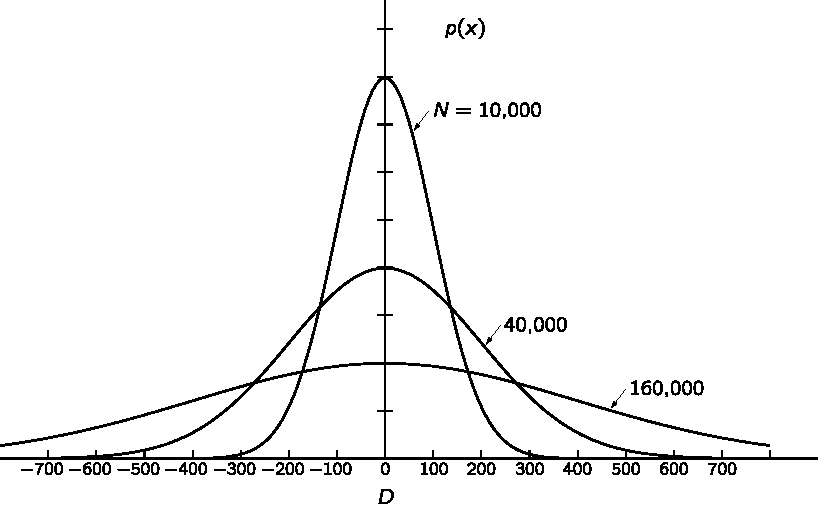
\includegraphics[width=0.55\textwidth]{Chapter6/在步数为N的无规行走中停止在从起点算起的距离}
    \caption{\footnotesize 在步数为$N$的无规行走中停止在从起点算起的距离$D$处的概率密度($D$是用方均根步长的单位来量度的)}
    \label{figure:在步数为N的无规行走中停止在从起点算起的距离}
\end{figure}

你们可能也已注意到,靠近零处的$p(x)$值反比于$\sqrt{N}$。这是由于曲线都有相似的形状以及曲线下面的面积都应相等而来的。既然$p(x)\Delta x$是当$\Delta x$很小时在$\Delta x$中找到$D$的概率,那么我们可以这样来确定在任意一个从$x_1$到$x_2$的间隔内\uwave{不论何处}找到$D$的概率,只要把间隔分割成许多微小增量$\Delta x$,然后对每个增量的有关概率$p(x)\Delta x$相加而求其总和。$D$落在$x_1$与$x_2$之间某处的概率,我们可以写作$P(x_1 < D < x_2)$,它等于图6.8中所示阴影的面积。增量$\Delta x$取得越小,结果就越正确。因此我们可以写成
\begin{equation}
\label{Eq:I:6:18}
P(x_1 < D < x_2)=\sum p(x)\,\Delta x=\int_{x_1}^{x_2}p(x)\,dx.
\end{equation}

\begin{wrapfigure}{r}{0.5\textwidth}
    \centering
    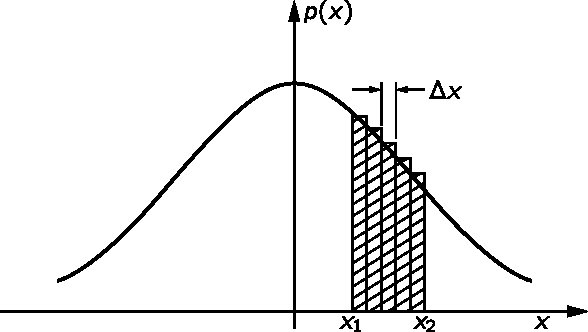
\includegraphics[width=0.35\textwidth]{Chapter6/无规行走中所通过的距离D,它位于x1与x2}
    \caption{\footnotesize 无规行走中所通过的距离$D$,它位于$x_1$与$x_2$之间的概率就是曲线$p(x)$下面从$x_1$到$x_2$的面积}
    \label{figure:无规行走中所通过的距离D,它位于x1与x2}
\end{wrapfigure}
整个曲线下面的面积是$D$落在不论何处(也就是它具有在$x=-\infty$到$x=+\infty$之间的\uwave{某一}值)的概率。这个概率当然是1。因而必须有
\begin{equation}
\label{Eq:I:6:19}
\int_{-\infty}^{+\infty}p(x)\,dx=1.
\end{equation}
由于图6.7中的曲线与$\sqrt{N}$成比例变宽,所以为了保持总面积等于$1$,它们的高度必须正比于$1/\sqrt{N}$。

我们这里所描述的概率密度函数是最经常遇到的一种,通常把它称为\uwave{正常}或\uwave{高斯}概率密度。它的数学形式是
\begin{equation}
\label{Eq:I:6:20}
p(x)=\frac{1}{\sigma\sqrt{2\pi}}\,e^{-x^2/2\sigma^2},
\end{equation}
其中$\sigma$称为\uwave{标准偏差},在我们的情况中$\sigma=\sqrt{N}$,或者当方均根步长不为1时,$\sigma=\sqrt{N}S_{\text{rms}}$。

前面我们已提到,气体中一个分子或任何一个粒子的运动犹如一种无规行走。假定我们打开一个装着有机化合物的瓶子,让它的一部分蒸气跑到空气中去。如果外面有气流,以致空气在作循环运动,那么气流也将带着蒸气一起运动。然而即使在\uwave{完全静止的空气}中,蒸气也会渐渐散布开去,进行扩散,直到布满整个空间。我们可以从它的颜色或气味加以鉴别。有机化合物蒸气的个别分子之所以能在静止空气中散布出去,是由于这些分子与其他分子碰撞而造成的分子运动所致。如果我们知道其“步子”的平均大小,以及每秒所走的步子,那么就能求出一个或$n$个分子在经过任何一段特定时间后在从其起点算起的某一距离被找到的概率。随着时间的消逝,步子越走越多,气体就会像图6.7中相继的几条曲线那样逐渐散开。在以后要讲的一章中,我们将求出步子的大小和步子的频率如何与气体的温度和压强有关。

我们以前说过,气体的压强是由于分子撞击容器壁而形成的。以后如果要作较定量的描写时,我们就需要知道分子在弹跳时跳得有多快,因为它们所作的碰撞与这个速率有关。然而我们不能说这些分子具有如何如何\uwave{确定的}速率,这里必须用概率来描写。一个分子可以具有任何一个速率,但有些速率出现的可能性比另一些要大。我们可以这样来描写气体内正在发生什么,这就是说处任何一个特定分子具有速率在$(v)$与$(v+\Delta v)$之间的概率$p(v)\,\Delta v$,而$p(v)$这个概率密度是速率$v$的一个确定函数。往后我们会看到,麦克斯韦如何运用常识和概率观念为$p(v)$找到一个数学表示式。函数$p(v)$的形状\footnote{麦克斯韦的表达式是$p(v)=Cv^2e^{-av^2}$,其中$a$是一个与温度有关的常数,而$C$应如此来选定,使总的概率等于$1$。}如图6.9所示。速度可以取任何一个值,但是最可能取的是靠近最可几值或预期值$\left < v \right >$的那一些。

\begin{wrapfigure}{r}{0.45\textwidth}
    \centering
    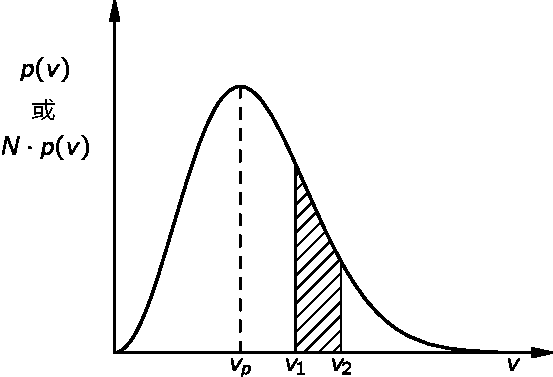
\includegraphics[width=0.35\textwidth]{Chapter6/气体中分子的速度分布}
    \caption{气体中分子的速度分布}
    \label{figure:气体中分子的速度分布}
\end{wrapfigure}

我们常常以稍微不同的方式去看待图6.9中的曲线。如果我们考虑一个典型容器(比如,其体积为1升)中的分子,那么容器中存在着极大数量的分子($N\approx10^{22}$)。由于$p(v)\,\Delta v$是\uwave{一个}分子具有在$\Delta v$间隔内的速度的概率,所以根据我们对概率的定义,我们说,找速度处在间隔$\Delta v$内的分子数其\uwave{预期值}$\left <\Delta N \right >$应是
\begin{equation}
\label{Eq:I:6:21}
\left <\Delta N\right >=N\,p(v)\,\Delta v.
\end{equation}
我们称$Np(v)$为“速度分布”。曲线下面两个速度$v_1$与$v_2$之间的面积,例如图6.9中所示阴影的面积代表了[对曲线$Np(v)$来说]速度在$v_1$和$v_2$之间的分子的预期数。由于在气体的情况中,我们通常与大量的分子打交道,所以可以期望这一面积与预期数的偏差是小的(犹如$1/\sqrt{N}$),因此我们常常不说“预期”数,代而说之:“具有速度在$v_1$和$v_2$之间的分子数\uwave{是}曲线下面的面积。”但是我们应当记住,这种陈述所谈到的总是\uwave{可几}数(probable numbers)。


\section{测不准原理}

在描写气体样品中$10^{22}$个或类似这样多个分子的行为时,概率的概念肯定是非常有用的。因为很清楚,即使要写下每个分子的位置或速度,这种试图也是不实际的,当概率最初运用这类问题时,大家曾认为这是一种\uwave{方便}——一种处理非常复杂的情况的方法。现在我们认为,概率的概念是描写原子事件所\uwave{必不可少}的。按照量子力学这个有关粒子的数学理论,在\uwave{说明}位置和速度方面总是存在着某种不确定性。充其量我们可以说,任何粒子只有一定的概率可以使它的位置接近某一坐标$x$。

我们可以这样来引进一个概率密度函数$p_1(x)$,使$p_1(x)\Delta x$为在$(x)$与$(x+\Delta x)$之间找到这个粒子的概率。如果这个粒子的位置被很好地限制在某个地方,比如说靠近$x_1$,那么函数$p_1(x)$就可能如图6.10(a)所示的曲线给出的那样。与之相似,我们必须用概率密度$p_2(v)$来限定粒子的速度,而$p_2(v)\Delta v$则表示能找到一个处于$v$与$v+\Delta v$之间的速度的概率,如图6.10(b)所示。

\begin{wrapfigure}{r}{0.45\textwidth}
    \centering
    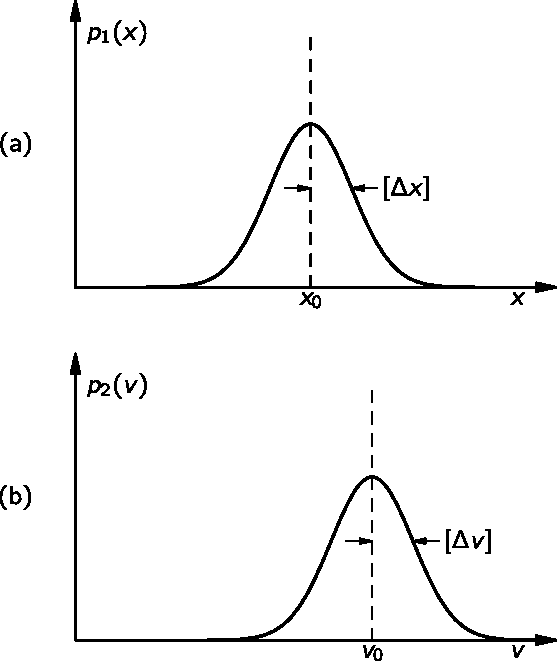
\includegraphics[width=0.35\textwidth]{Chapter6/观察一个粒子的位置与速度时的概率密度}
    \caption{观察一个粒子的位置与速度时的概率密度}
    \label{figure:观察一个粒子的位置与速度时的概率密度}
\end{wrapfigure}

量子力学的基本结果之一是:两个函数$p_1(x)$与$p_2(v)$不能予以独立选定,特别是不能把它们都取得任意的窄。如果我们称$p_1(x)$曲线的典型“宽度”为$[\Delta x]$,$p_2(v)$曲线的典型宽度为$[\Delta v]$(各如图所示),那么自然界就要求这两个宽度的乘积至少要与数$\hbar/2m$,其中$m$是粒子的质量。我们可以把这个基本关系写成
\begin{equation}
\label{Eq:I:6:22}
[\Delta x]\cdot[\Delta v]\geq\hbar/2m.
\end{equation}

这个式子就是我们前面提到过的\uwave{海森堡测} \uwave{不准原理}的一种表述。

由于式(6.22)的右面是一个常数,这就表明,如果我们迫使一个粒子处于某一特定位置而试图把它“钉住”,结果它就获得一个很大的速度。或者是:如果我们迫使它跑得很慢,或以精确的速度运动,那么它就要“散开”,以致我们不能很好地知道它究竟在那里。粒子的举止真是太奇妙了!

测不准原理描述了在叙述自然界的任何尝试中所必然存在着的那种内在的模糊性或不明确性。我们对自然界的最准确描写必须用\uwave{概率}的观念。有些人不喜欢用这种方法来描写自然界,不知怎么地,他们总觉得,只要能说出一个粒子\uwave{真正}在做什么,他们就能同时知道它的速度和位置。在量子力学发展的初期,爱因斯坦曾为这个问题十分担忧。他常摇头说:“啊!上帝肯定不是用掷骰子来决定电子应如何运动的!”他为这个问题担忧了好长时间,或许他从来也没有使他自己真正相信过这个事实,即:这是人们对自然界所能作出的最好描述。现在仍然有一、二位物理学家在研究这问题,他们从直觉上深信,可以通过某种方式用另一种方法来描写这个世界,并且可以把有关事物行为的所有这种不确定性都消除掉。然而到现在没有一个成功的。

当我们希望描写原子结构时,确定一个粒子的位置所必然要出现的不确定性就变得极为重要。在氢原子中有一个由单个质子组成的核,核的外面有一个电子,而这个电子的位置的不确定性就同原子本身一样大!因此我们不能严格地说:电子在某一“轨道”上绕质子运动,最多我们可以说,在一个离质子距离为$r$的体积元$\Delta V$内有一定的\uwave{机会}($p(r)\,\Delta V$)观察到这个电子,概率密度$p(r)$由量子力学来确定。对一个未受扰动的氢原子来说,$p(r)=Ae^{-2r/a}$,这是一个如图6.8所示的那种钟形函数。数$a$是“典型”的半径,函数由这里开始减小很快。既然在离原子核距离远大于$a$的地方找到电子的概率很小,我们可以把$a$设想为“原子的半径”,大约等于$10^{-10}$米。

\begin{wrapfigure}{r}{0.45\textwidth}
    \centering
    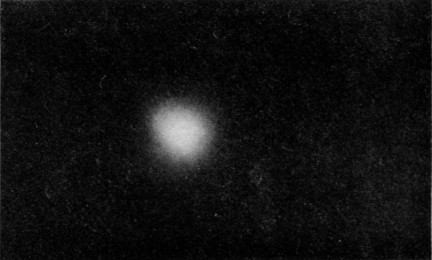
\includegraphics[width=0.35\textwidth]{Chapter6/使氢原子形象化的一种方法}
    \caption{\footnotesize 使氢原子形象化的一种方法。这里云的密度(洁白度)表示能观察到电子的概率密度}
    \label{figure:使氢原子形象化的一种方法}
\end{wrapfigure}
如果想像有这样一团“云”,它的密度正比于我们能观察到的电子的概率密度,那么我们就能形成氢原子的图象。这样一团云的一个实例如同6.11所示。所以我们对氢原子的最好“写照”便是一团“电子云”(虽然我们\uwave{实际}上指的是“概率云”)围绕着一个核。电子就处在云中某一地方,但自然界只允许我们知道在任何一个特定位置上能找到它的\uwave{机会}是多少。

在尽可能多地了解自然界的努力中,现代物理学曾发现,有些事情永远不可能确切地“知道”。我们的许多知识必然总是不确定的,而用概率来表述时,我们所能获得的知识则\uwave{最多}。
